In chapter~\ref{ch:mvica1}, we have introduced MultiViewICA and presented its
theoretical properties.
In this chapter, we empirically verify through extensive experiments on fMRI and
MEG data that MultiView ICA improves component identification with respect to competing methods, suggesting that the expressiveness and robustness of this model make it a useful tool for multivariate neural signal analysis.

\section{Experimental setting}
\label{sec:expts}
In the following, the noise parameter in MultiviewICA is always fixed to $\sigma =1$.
We use the function $f(\cdot)= \log\cosh(\cdot)$, giving the non-linearity $f'(\cdot) = \tanh(\cdot)$.
We use the Infomax cost function~\cite{bell1995information} with the same non-linearity to perform standard ICA, with the Picard algorithm~\cite{ablin2018faster} for fast and robust minimization of the cost function. Picard is applied with the default hyper-parameters.
The code for MultiViewICA is available online at \url{https://github.com/hugorichard/multiviewica}.
%

We compare the following methods to obtain $p$ components:
\emph{PermICA} is described in section~\ref{sec:permica}.
%
\emph{SRM} is the FastSRM algorithm described in part~\ref{part:fastsrm}.
%
\emph{ConcatICA} is described in section~\ref{sec:canicaandconcatica}.
%
\emph{PCA+ConcatICA} corresponds to ConcatICA applied on subject data that have been first individually reduced by PCA with $p$ components. 
%
\emph{CanICA} is described in section~\ref{sec:canicaandconcatica}.
We define the chance level as the performance of an algorithm that computes unmixing matrices and projections to lower dimensional space by sampling random numbers from a standard normal distribution. 
% 


The dimension reduction in MultiView ICA and PermICA is performed with SRM in
fMRI experiments and subject-specific PCA in MEG experiments.

Since the cost function $\mathcal{L}$ is non-convex, having a good initialization can make a difference in the final result. We propose a two stage approach.
We begin by applying PermICA on the datasets, which gives us a first set of unimixing matrices $W_1, \dots, W_m$.
Note that we could also use ConcatICA for this task.
Next, we perform a diagonal scaling of the mixing matrices, i.e. we find the diagonal matrices $\Lambda_1, \dots, \Lambda_m$ such that $\mathcal{L}(\Lambda_1W_1, \dots, \Lambda_mW_m)$ is minimized.
To do so, we employ Algorithm~\ref{algo:mv_ica} but only take into account the diagonal of the descent direction at each step: the update rule becomes $W_i \leftarrow (I_p + \rho \text{Diag}(D))W_i$.
The initial unmixing matrices for Algorithm~\ref{algo:mv_ica} are then taken as $\Lambda_1W_1, \dots, \Lambda_mW_m$.
Empirically, we find that this two stage procedure allows for the algorithm to start close from a satisfactory solution.
A summary of our quantitative results on real data is available in appendix~\ref{sec:app_real_data}.


\section{Synthetic experiment}

We validate our method on synthetic data generated according to the model in equation~\eqref{eq:ica_model}.
%
The components are generated i.i.d. from a Laplace density $d(x)=\frac12\exp(-|x|)$.
%
The mixing matrices $A_1,\cdots, A_m$ are generated with i.i.d. entries following a normal law.
Each compared algorithm returns a sequence of estimated unmixing matrices $W_1, \dots, W_m$.
%
The performance of an algorithm is measured by the reconstruction error between the estimated components and the true components.

\begin{figure}
  \label{fig:synth}
  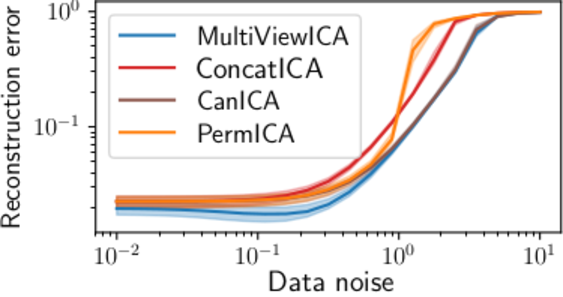
\includegraphics[width=0.5\textwidth]{figures/mvica/distance_expe.pdf}
  \captionof{figure}{\textbf{Synthetic experiment}: reconstruction error of the algorithms on data following model~\eqref{eq:ica_model}.}
\end{figure}

%$\frac1M\sum_{i=1}^Md(W^iA^i)$, where $d(P)=\sum_{i=1}^n \left(\sum_{j=1}^n\frac{|p_{ij}|}{\max_{p} |p_{ip}|} - 1\right) + \sum_{j=1}^n \left(\sum_{i=1}^n\frac{|p_{ij}|}{\max_{p} |p_{pj}|} - 1\right)$.
%
%This quantity cancels if and only if $P$ is a scale and permutation matrix.
%
We use $m=10$ datasets, $p=15$ components and $n=1000$ samples. Each experiment is repeated with $100$ random seeds.
%
We vary the noise level in the data generation from $10^{-2}$ to $10$.

Multiview ICA has uniformly better performance than the other algorithms, which illustrates the strength of maximum-likelihood based methods. In accordance with results of section~\ref{sec:mvica}, it is able to separate the components even with misspecified noise parameter and component density.
%
%\subsection{fMRI experiments}
%\label{sec:experiments}


\section{fMRI experiments}
We use the \emph{Forrest} and \emph{Sherlock} datasets described in section~\ref{srm:datasets:fmri}.
We also add two other datasets:

The \emph{RAIDERS} dataset reproduces the protocal described
in~\cite{haxby2011common}. 10 participants are watching the movie "Raiders
of the lost ark". This dataset pertains to the Individual Brain Charting
dataset~\cite{ibc}.
% 
Data 
% 
We use full brain data of 10 subjects split in 9 runs of respectively 374, 297, 314, 379, 347, 346, 350, 353 and 211 timeframes.
%
Note that the Raiders dataset is different from the one used in~\cite{chen2015reduced}, as it involves different subjects, and because data were acquired at NeuroSpin using a 3T scanner with an isotropic spatial resolution of 1.5 mm.
The \emph{raiders-full} dataset~\cite{ibc} is an extension of the \emph{raiders} dataset where the first two scenes of the movie are shown twice (130 mins).

The CLIPS dataset reproduces the protocol of original studies described in
\cite{nishimoto2011reconstructing} and \cite{huth2012continuous}. 10
participants are exposed to short clips. The data were acquired in 17 runs of 325 timeframes. 
%
The CLIPS dataset also pertains to the Individual Brain Charting dataset (\cite{ibc}) and reproduces .
%
At the time of writing, the CLIPS and RAIDERS dataset from the individual brain charting dataset \url{https://project.inria.fr/IBC/} are not yet public, but they will be in the future. Protocols on the visual stimuli presented are available in a dedicated repository on Github: \url{https://github.com/hbp-brain-charting/public_protocols}.

A summary about the size of each dataset is available in Table~\ref{tab:dataset_desc}.
\begin{table}
	\begin{tabular}{|c|c|c|c|c|}
		\hline
		\textbf{Dataset} & \textbf{Subjects} & \textbf{Runs} & \textbf{Average run} & \textbf{Voxels} \\
                     && & \textbf{length} & \textbf{(per subject)} \\
                     && & \textbf{(in timeframes)} &  \\
                     &$m$& $ $ & $n$ &$v$  \\
		\hline
		CLIPS & 10 & 17 & 325 & 212445\\ 
		\hline
		SHERLOCK & 16 & 5 & 395 & 212445 \\ 
		\hline
		RAIDERS & 10 & 9 & 330 & 212445 \\
		\hline 
		FORREST & 19 & 7 & 465 & 212445\\
		\hline
		CamCAN & 647 & 1 & 193 & 212445 \\
		\hline
	\end{tabular}
  \caption{\textbf{Datasets description}}
  \label{tab:dataset_desc2}
\end{table}

%
%
The preprocessing is the same as the one described in section~\ref{srm:datasets:fmri}.
Unless stated otherwise we use spatially unsmoothed data, except for the \emph{sherlock} dataset, for which the available data are already preprocessed with a 6\,mm spatial smoothing.

\subsection{Reconstructing the BOLD signal of missing subjects}
\label{sec:srm:reconstruction}
\label{reconstruction}
We want to show that once unmixing matrices have been learned, they can be
used to predict evoked responses across subjects. This can be used to perform
missing data imputation when the sessions of some subjects are missing.
In~\cite{zhang2018transfer}, the authors consider multiple fMRI datasets that
share a subpart of their subjects and use the fact that some subjects are shared
to transfer information across datasets. Our reconstruction experiment measures
a related quantity: the methods ability to predict data of left-out subjects
from other subjects.

In this experiment we apply a 6\,mm spatial smoothing to all datasets. 
We split the data into three groups. First, we randomly choose $80\%$ of all runs from all subjects to form the training set.
%
Then, we randomly choose $80\%$ of subjects and take the remaining $20\%$  runs as testing set.
%
The left-out runs  of the remaining $20\%$ subjects form the validation set.
%
The compared algorithms are run on the training set and evaluated using the testing and validation sets.
%
After an algorithm is run on training data, it defines for each subject a \emph{forward operator} that maps individual data to the component space and a \emph{backward operator} that maps the component space to individual data. For instance in ICA the forward operator is the product of the dimensionality reduction projection and unmixing matrix.
%
We estimate the shared responses on the testing set by applying the forward operators on the testing data and averaging. Finally, we reconstruct the individual data from subjects in the validation set by applying the backward operators to the shared responses. We measure the difference between the true signal and the reconstructed one using voxel-wise $R^2$ score. The $R^2$ score between two series $\xb \in \bbR^n$ and $\yb \in \bbR^n$ is defined as
$R^2(\xb, \yb) = 1 - \frac1{n\Var(\yb)}\sum_{t=1}^n (x_t - y_t)^2$, where $\Var(\yb) = \frac1n\sum_{t=1}^n (y_t - \frac1n \sum_{t'=1}^n y_{t'})^2$ is the empirical variance of $\yb$.
%
The $R^2$ score is always smaller than $1$, and equals $1$ when $\xb= \yb$.
The experiment is repeated 25 times with random splits to obtain error bars.

An illustration of our reconstruction experiment is available in Figure~\ref{fig:experiment_reconstruction}.

\begin{figure}
  \centering
  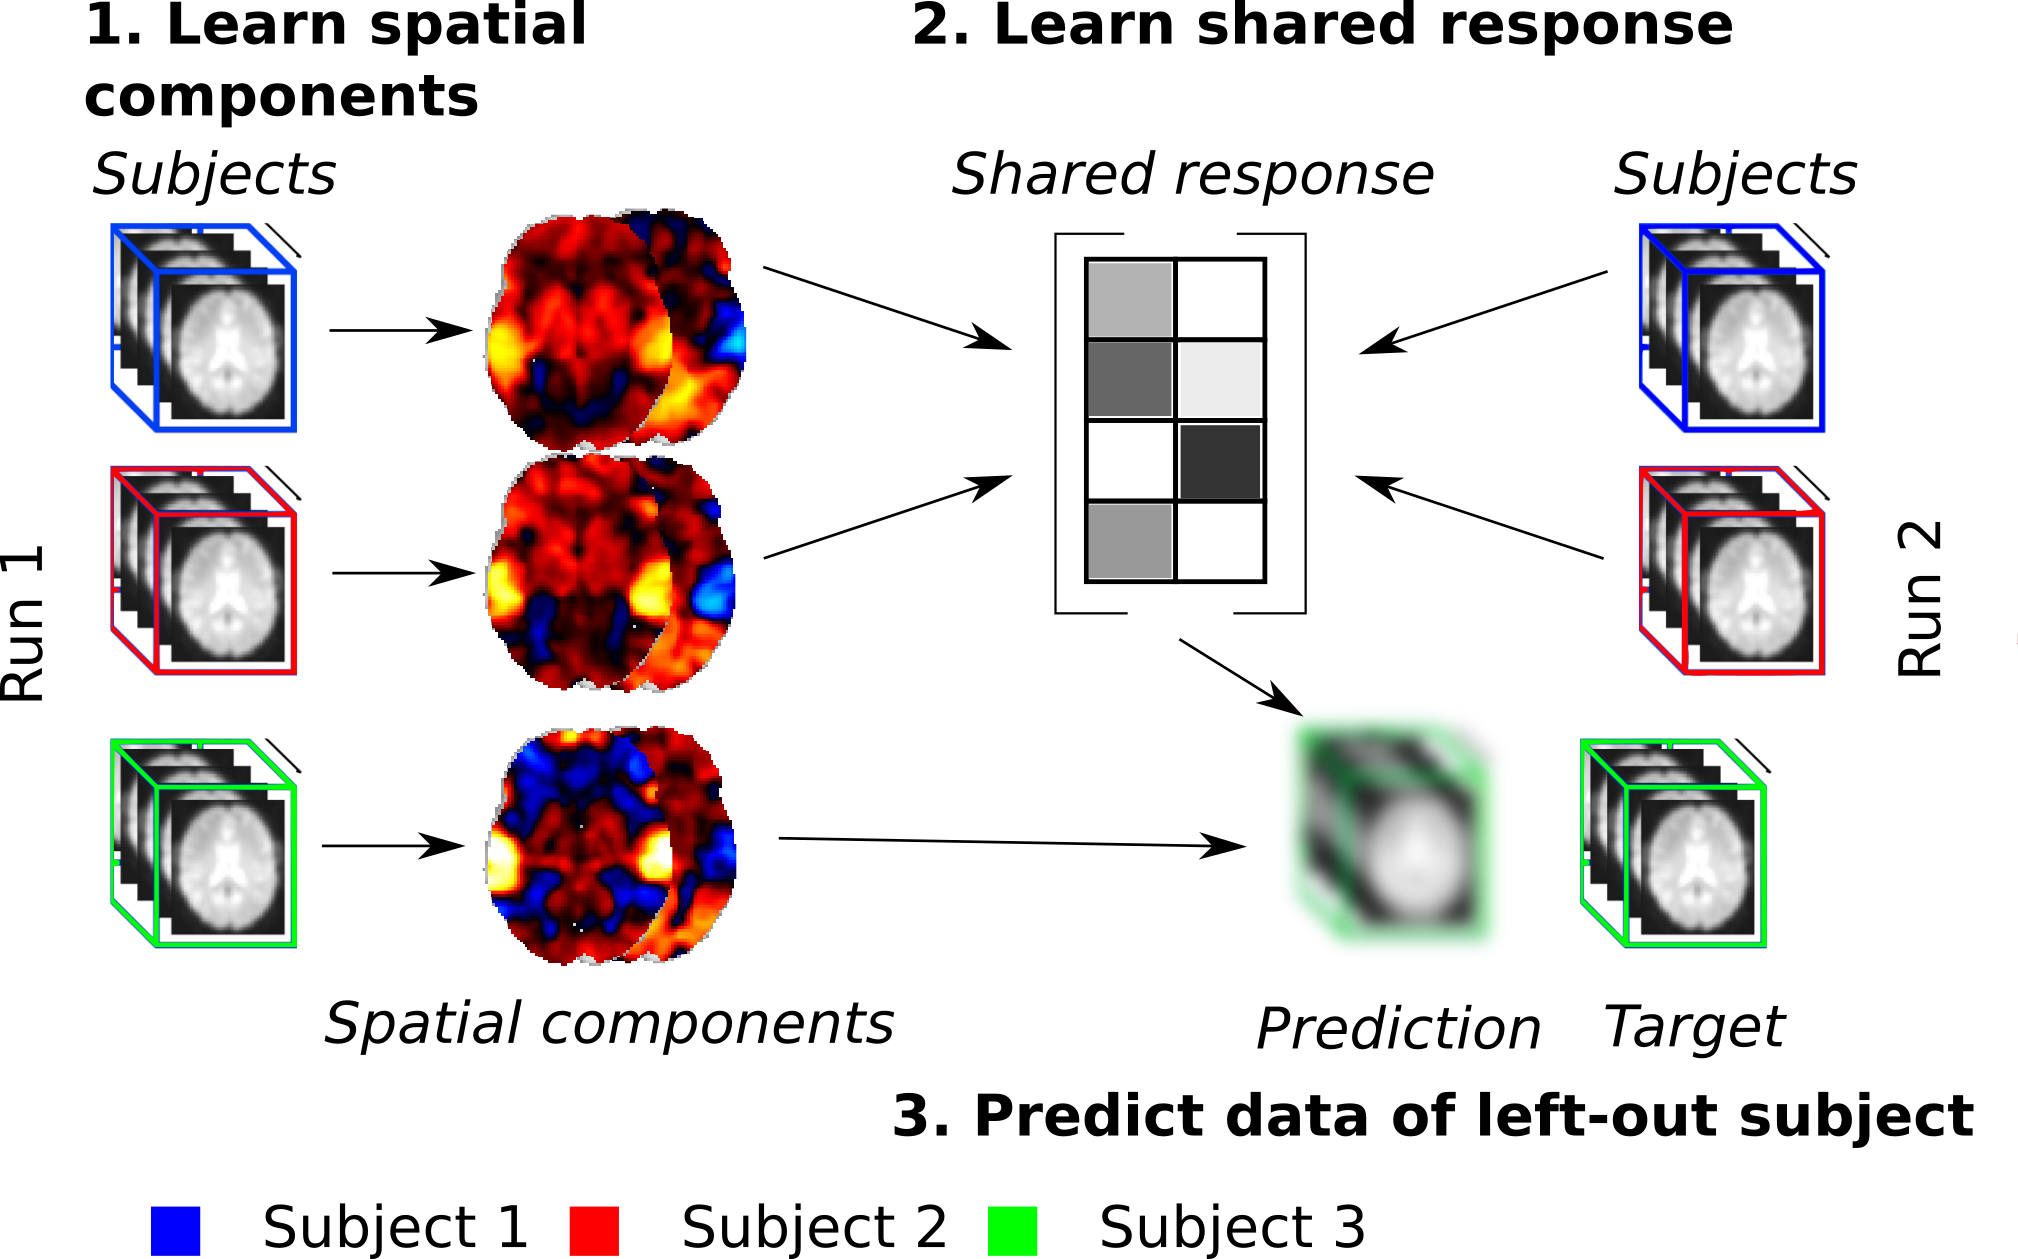
\includegraphics[scale=0.24]{figures/srm/conceptual_figure41.png}
  \caption{\textbf{Experiment — Reconstruct data from a left-out subject} All runs but one are used to compute spatial components for every subject (left).
    % 
    Then spatial components and data from the left-out run of all subjects but one are used to compute the shared response in the left-out run.
    % 
    At last, the shared response during the left-out run and  the spatial components of the test subject are used to predict the data of the test subject in the left-out run.
    % 
    The performance of the model is measured by comparing the prediction and true data using the $R^2$ score.}
  \label{fig:experiment_reconstruction}
\end{figure}


The $R^2$ score per voxel depends heavily on which voxels are considered. For example voxels in the
visual cortex are better reconstructed in the \emph{sherlock} dataset than in
the \emph{forrest} dataset.

Performances are therefore given in terms of mean $R^2$ score inside a region of interest (ROI) in order to leave out regions where there is no useful information.

In order to determine the ROIs, we focus on the R2 score per voxel between the BOLD signal reconstructed by ConcatICA and the actual bold signal. We run ConcatICA with $10, 20$ and $50$ components and select the voxels that obtained a positive R2 score for all sets of components.
% 
We discard voxels with an R2 score above 80\% as they visually correspond to artefacts and apply a binary opening using a unit cube as the structuring element. The chosen regions are plotted in figure~\ref{fig:roi}.

\begin{figure}
  \centering
  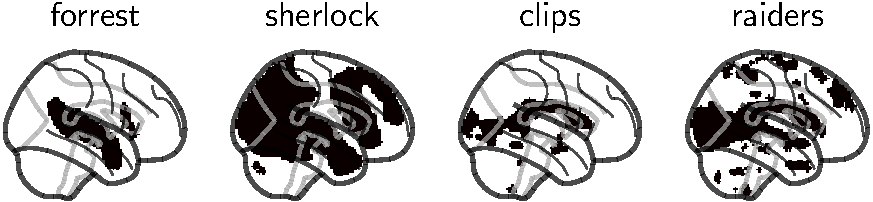
\includegraphics[width=\textwidth]{figures/mvica/reconstruction_score_roi.pdf}
  \caption{\textbf{Data-driven choice of ROI} Chosen ROIs for the experiment: Reconstructing the BOLD signal of missing subjects.}
  \label{fig:roi}
\end{figure}

 In Figure~\ref{fig:reconstruction}
(top) we report the mean $R^2$ score inside region of interest.
%
MultiView ICA has similar or better performance than the other methods on all datasets.
%
This demonstrates its ability to capture inter-subject variability, making it a candidate of choice to handle missing data or perform transfer learning.

\begin{figure}
  \centering
  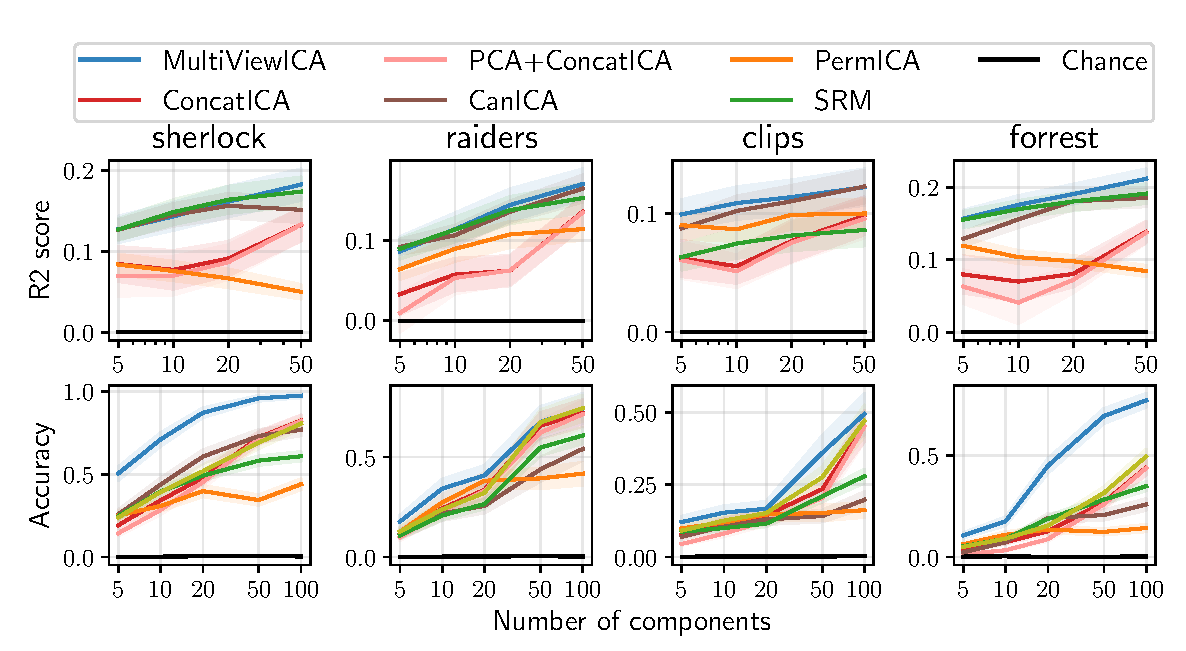
\includegraphics[width=0.9\textwidth]{figures/mvica/timesegment_matching_reconstruction.pdf}
  \caption{\emph{Top:} \textbf{Reconstructing the BOLD signal of
      missing subjects}. Mean $R^2$ score between reconstructed data and true
    data (higher is better). \emph{Bottom:} \textbf{Between subjects time-segment matching}. Mean
    classification accuracy. Error bars represent a 95 \% confidence interval over cross validation splits.}
  \label{fig:reconstruction}
  \label{fig:timesegment}
\end{figure}


For completeness, we plot in Figure~\ref{fig:brainmaps}, for ConcatICA, SRM and MultiViewICA, the R2 score per voxel using 50 components for datasets \emph{sherlock}, \emph{forrest}, \emph{raiders} and \emph{clips}. As could be anticipated from the task definition, \emph{forrest} obtains high reconstruction accuracy in the auditory cortices, while \emph{clips} shows good reconstruction in the visual cortex (occipital lobe mostly); the richer \emph{sherlock} and \emph{raiders} datasets yield good reconstructions in both domains, but also in other systems (language, motor).
%
We also see visually see that data reconstructed by MultiViewICA are
a better approximation of the original data than other methods.
%
This is particularly obvious for the \emph{clips} datasets where it is
clear that voxels in the posterior part of the superior
temporal sulcus are better recovered by MultiViewICA than by SRM or
ConcatICA.

\begin{figure}
  \centering
  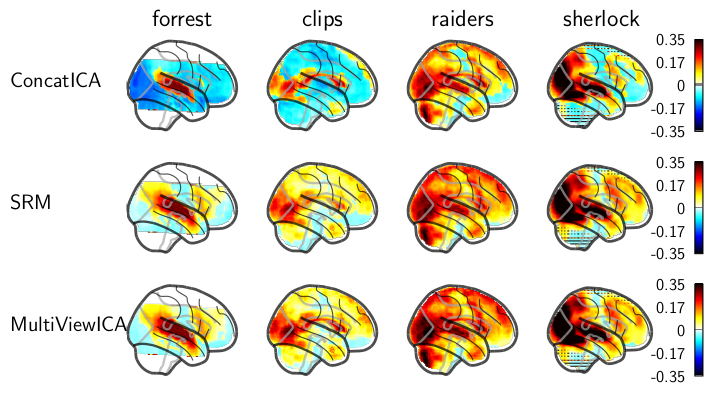
\includegraphics[width=\textwidth]{figures/mvica/reconstruction_score_fullbrain.png}
  \caption{\textbf{Reconstructing the BOLD signal of missing subjects: Reconstruction R2 score per voxel} We plot for ConcatICA, SRM and MultiViewICA, the R2 score per voxel using 50 components for datasets \emph{sherlock}, \emph{forrest}, \emph{raiders} and \emph{clips}. We visually see that data reconstructed by MultiViewICA are more faithful reproduction of the original data than other methods.}
  \label{fig:brainmaps}
\end{figure}

%
\subsection{Between subjects time-segment matching} 
We reproduce the time-segment matching experiment in
section~\ref{sec:timesegment_expe}. 
MultiView ICA yields a consistent and substantial improvement in accuracy compared to other methods on the four datasets. We see a marked improvement on the datasets sherlock and forrest. A possible explanation lies in the preprocessing pipeline. Sherlock data undergo a 6~mm spatial smoothing and Forrest data are acquired at a higher resolution (7T vs 3T for other data). This affects the signal to noise ratio.
%

In order to investigate the practical impact of the choice of hyper-parameter
$\sigma$, we compute the accuracy of the MultiView ICA algorithm with different
choice of $\sigma$.
Results are reported in Fig.~\ref{fig:supp_noise_sensitivity}. 
\begin{figure}
  \centering
  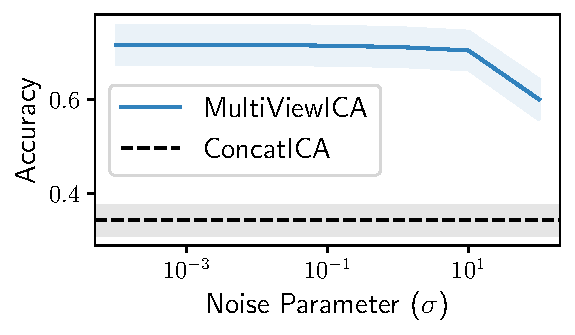
\includegraphics[width=0.6\textwidth]{figures/mvica/noise_sensitivity.pdf}
  \caption{\textbf{Effect of the parameter $\sigma$}: We compute the accuracy of the multiview-ICA pipeline on the time-segment matching experiment for various values of the $\sigma$ hyperparameter over a grid. The accuracy varies only marginally with $\sigma$.}
  \label{fig:supp_noise_sensitivity}
\end{figure}
MultiviewICA performs consistently well for a wide range of noise parameter values, and only breaks at very high values. It supports the theoretical claim of Prop~\ref{prop:robust} that the noise parameter is of little importance.

In appendix~\ref{sec:spatial_maps}, we plot the average forward operator across subjects of MultiView ICA and ConcatICA with 5 components on the forrest, sherlock, raiders and clips datasets.


\subsection{Between-runs time-segment matching}
\label{app_spatialmaps}
We measure the ability of each algorithm to extract meaningful shared components that correlate more when they correspond to the same stimulus than when they correspond to distinct stimuli. We use the \emph{raiders-full} dataset, which allows this kind of analysis because subjects watch some selected scenes from the movie twice, during the first two runs (1 and 2) and the last two (11 and 12).
%
First, the forward operators are learned by fitting each algorithm with 20 components on the data of all 11 subjects using all 12 runs. We then select a subset of 8 subjects and the shared components are computed by applying the forward operators and averaging.
%
We select a large target time-segment ($50$
timeframes) taken at random from run 1 and 2, and we try to localize the corresponding sample time-segment from the 10 last runs using a single component of the shared components.
%
The time-segment is said to be
correctly classified if the correlation between the target and corresponding sample
time-segment is higher than with any other time-segment (partially overlapping windows are excluded).
%
In contrast to the \emph{between subject time-segment matching} experiment, we obtain one accuracy score per component.
%
We repeat the experiment 10 times with different subsets of subjects randomly chosen and report the mean accuracy of the 3 best performing components in Figure~\ref{fig:swetha}. Error bars correspond to a 95~\% confidence interval.
%
MultiView ICA achieves the highest accuracy.

\begin{figure}
  \centering
  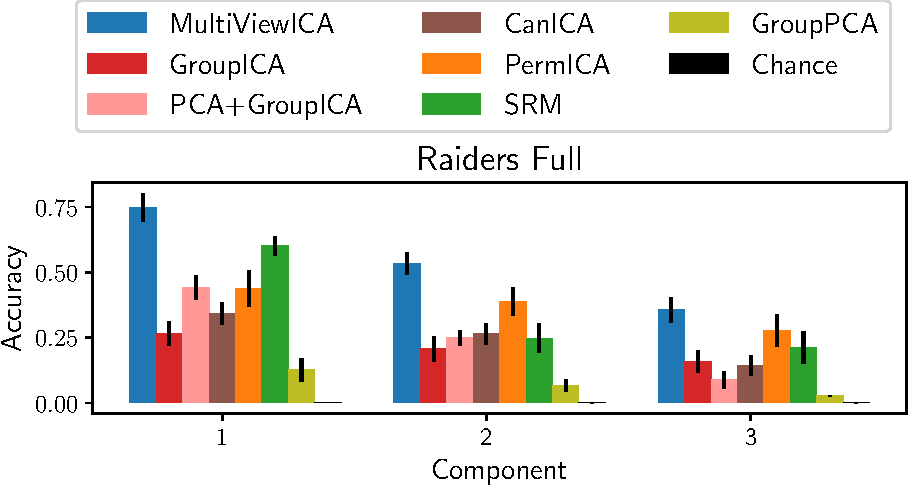
\includegraphics[width=\textwidth]{figures/mvica/swetha_exp_full_fit.pdf}
  \caption{\textbf{Between runs time-segment matching}. Interesting components correlates more when they correspond to the same stimulus (same scenes of the movie) than when they correspond to distinct stimuli (different scenes).
  %We show that when MultiView ICA is used, we can locate a target time-segment in one session using the data of another session corresponding to the same stimuli.
  We extract 20 components and report the mean accuracy of the 3 best performing components}
  \label{fig:swetha}
\end{figure}


We then focus on the 3 best performing components of MultiView ICA. For each component, we plot in Figure~\ref{fig:app_spatialmaps} (left) the shared components during two sets of runs where subjects were exposed to the same scenes of the movie. We then study the localisation of these components.
%
We average the forward operators across subjects and plot the columns corresponding to the components of interest in Figure~\ref{fig:app_spatialmaps} (right).
%
As each column is seen as a set of weights over all voxels, it represents a spatial map.

The component 1 of the shared responses follows almost the same pattern in the two set of runs corresponding to the same scenes of the movie. The spatial map corresponding to component 1 highlights the language network.
%
In component 2, the temporal patterns during the viewing of identical scenes are also very similar. The corresponding spatial map highlights the visual network especially the visual dorsal pathway.
%
In component 3, there exists a similarity however less striking than with the two previous components. The corresponding spatial map highlights a contrast between the spatial attention network and the auditory network.

\begin{figure}
  \centering
  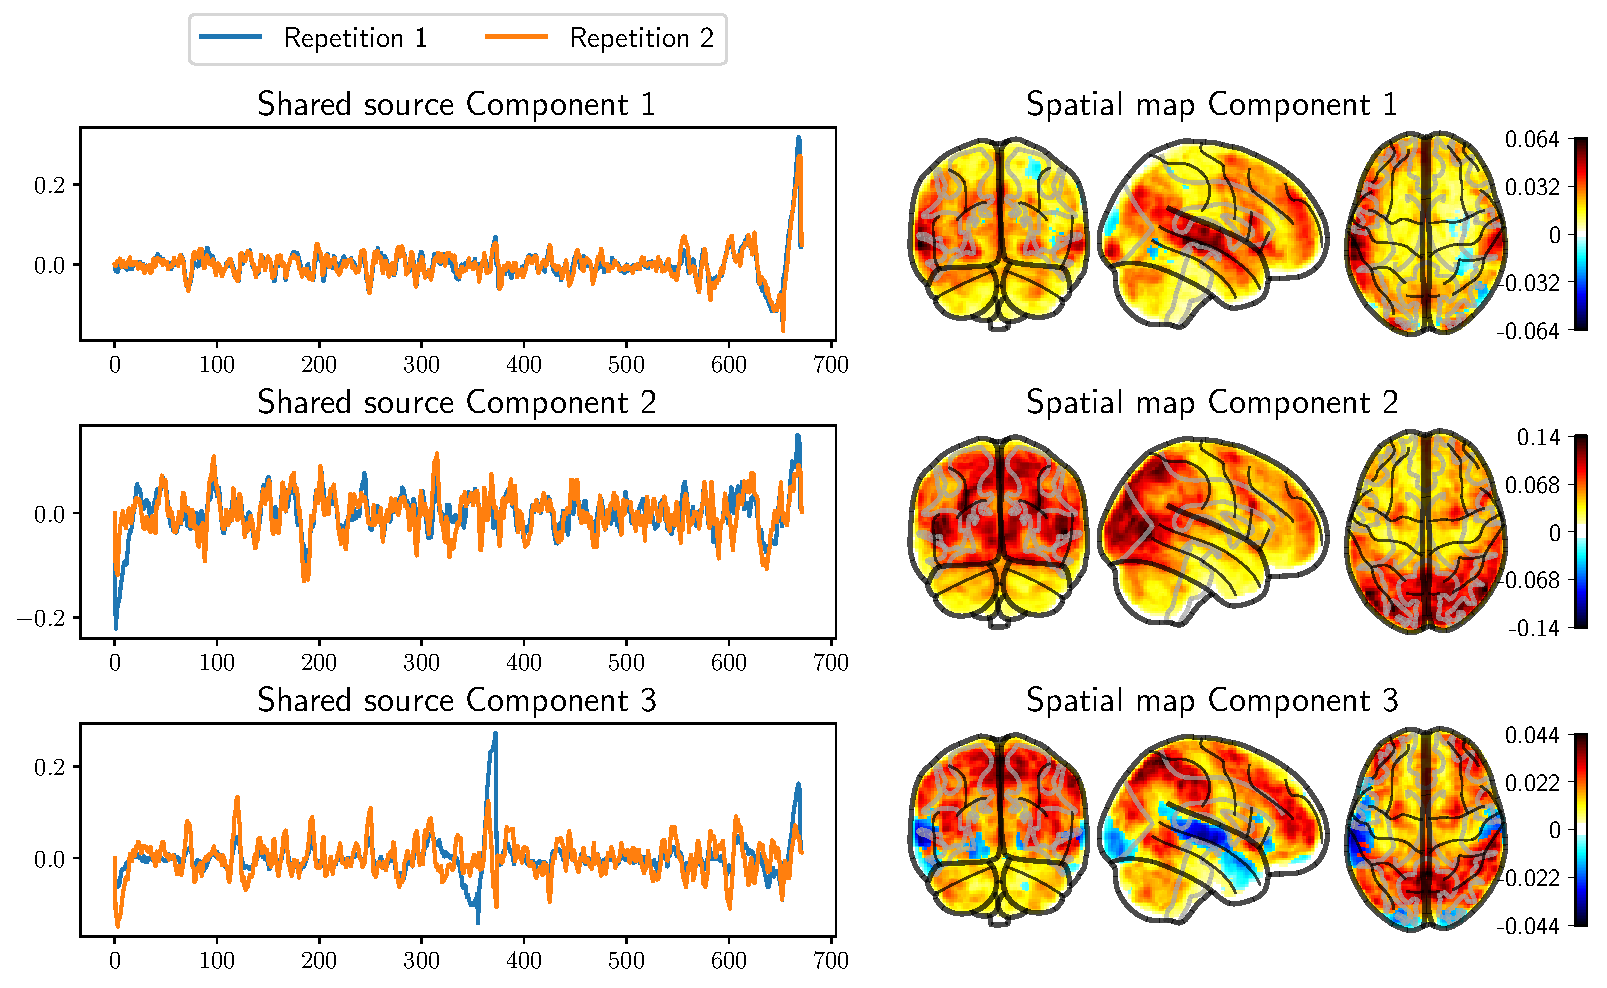
\includegraphics[width=\textwidth]{figures/mvica/swetha_exp_full_fit_appendix.pdf}
  \caption{\textbf{Between-runs time segment matching: spatial maps and timecourses} \emph{Left:} Timecourses of the 3 shared components yielding the highest accuracy. The two displayed set of runs correspond to the same scenes in the movie. \emph{Right:} Localisation of the same shared components in the brain}
  \label{fig:app_spatialmaps}
\end{figure}


%\subsection{MEG experiments}
\section{Phantom MEG data}
\label{sec:mvica:phantom}
We demonstrate the usefulness of our approach on MEG data.
%
The first experiment uses data collected with a realistic head phantom, which is a plastic device mimicking real electrical brain components.
%
Eight current dipoles positioned at different locations can be switched on or off.
%
We view each dipole as a subject and therefore have $m=8$.
%
We only consider the 102 magnetometers.
%
An epoch corresponds to 3\,s of MEG signals where a dipole is switched on for 0.4\,s with an oscillation at 20\,Hz and a peak-to-peak amplitude of 200\,nAm.
%
This yields a matrix of size $p\times n$ where $p=102$ is the number of sensors, and $n$ is the number of time samples.
%
We have access to $100$ epochs per dipole.
%
For each dipole, we chose $N_e=2, \dots, 16$ epochs at random among our set of 100 epochs and concatenate them in the temporal dimension.
%
We then apply algorithms on these data to extract $p=20$ shared components.
%
As we know the true component (the timecourse of the dipole), we can compute the reconstruction error of each component as the squared norm of the difference between the estimated component and the true component, after normalization to unit variance and fixing the sign.
%
We only retain the component of minimal error.
%
We also estimate for each forward operator the localization of the component by performing dipole fitting using its column corresponding to the component of minimal error.
%
We then compute the distance of the estimated dipole to the true dipole.
%
These metrics are reported in figure~\ref{fig:meg} when the number of epochs considered $N_e$ varies.
%
% We also compare our method to the Bayesian Canonical Correlation Analysis (BCorrCA) of~\cite{kamronn2015multiview}.
% %
% On this task, BCorrCA is outperformed by ICA methods.
%
MultiView ICA requires fewer epochs to correctly reconstruct and localize the true component.
%

\section{Experiment on Cam-CAN dataset}
Finally, we apply MultiView ICA on the Cam-CAN dataset~\cite{taylor2017cambridge}. We use the magnetometer data from the MEG of $200$ subjects.
%
Each subject is repeatedly presented an audio-visual stimulus. 
%
The MEG signal corresponding to these trials are then time-averaged to isolate the evoked response, yielding individual data.
%
The MultiView ICA algorithm is then applied to extract $20$ shared components.
%
$9$ components were found to correspond to noise by visual inspection, and the $11$ remaining are displayed in figure~\ref{fig:meg}.
%
We observe that MultiView ICA recovers a very clean sequence of evoked potentials with sharp peaks
for early components and slower responses for late components.
%
In order to visualize their localization, we perform component localization for each subject by solving the inverse problem using sLORETA~\cite{pascual2002standardized}, providing a component estimate for each component.
%
Then, we register each component estimate to a common reference brain.
%
Finally, the component estimates are averaged, and thresholded maps are displayed in figure~\ref{fig:meg}.
%
Individual maps corresponding to each component are displayed in appendix~\ref{sec:app_montages}.
The figure highlights both early auditory and visual cortices, also suggesting a propagation
of the activity towards the ventral regions and higher level visual areas.

\begin{figure}
    \centering

          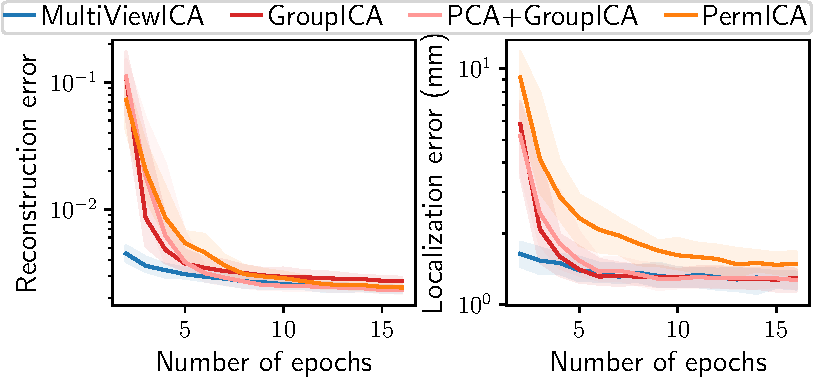
\includegraphics[width=0.6\textwidth]{figures/mvica/phantom.pdf}
          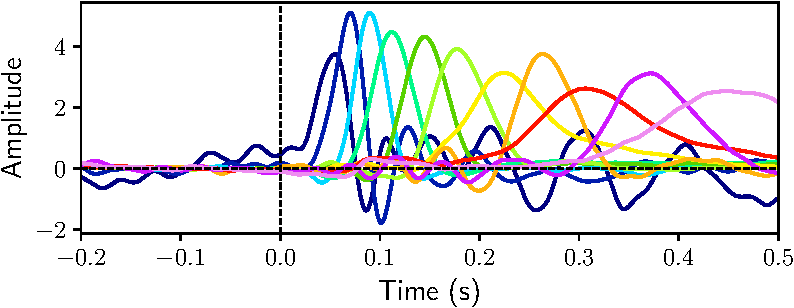
\includegraphics[width=0.6\textwidth]{figures/mvica/camcan_sources.pdf}
          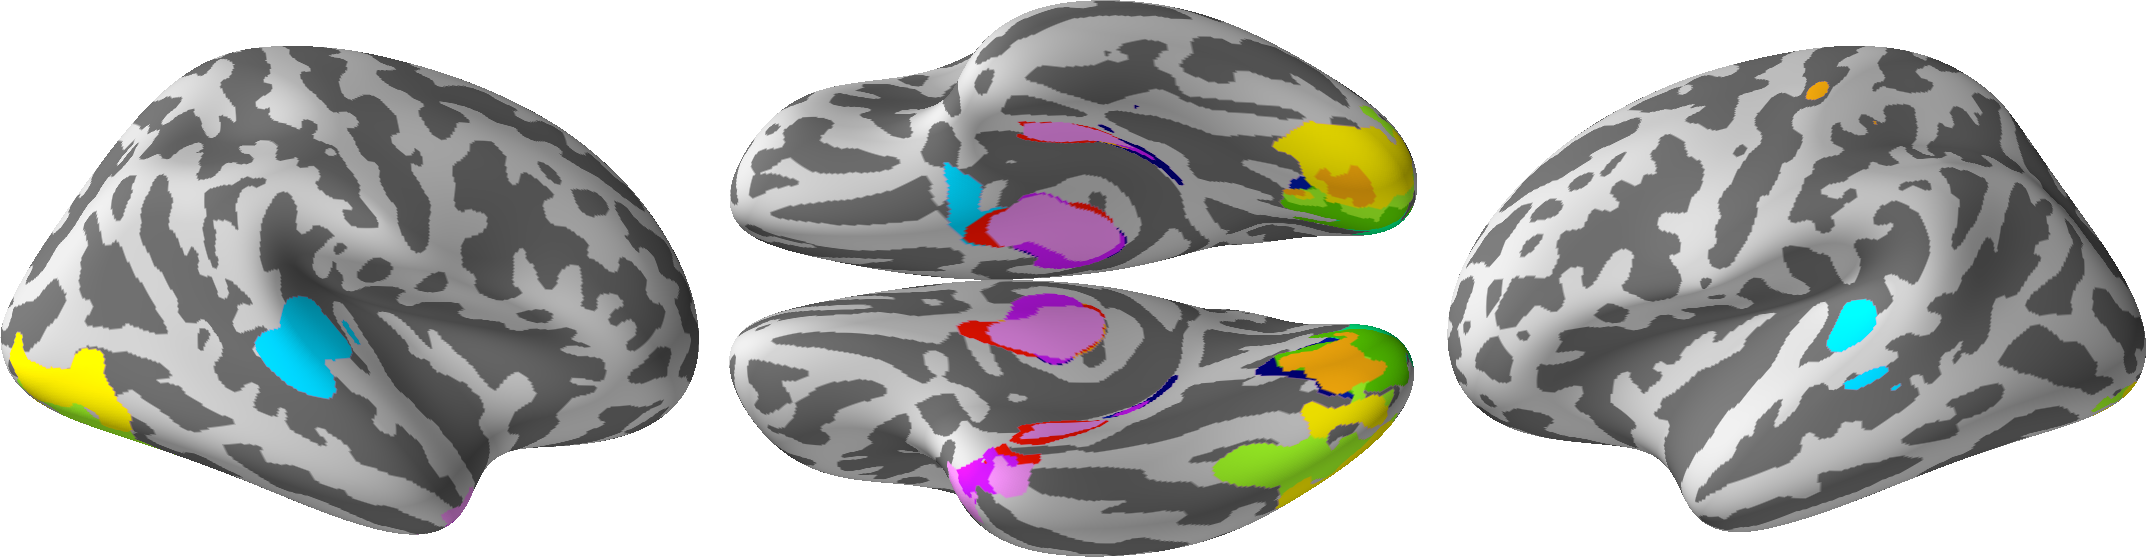
\includegraphics[width=0.6\textwidth]{figures/mvica/montage_all.png}
    \caption{\emph{Top:} \textbf{Experiment on MEG Phantom data}. Reconstruction
      error is the norm of the difference between the estimated and true
      component. Localization error is the distance between the estimated and
      true dipole. \emph{Middle and Bottom:} \textbf{Experiment on 200 subjects from the CAM-can dataset} \emph{Middle:} Time course of $11$ shared components (one color per component). We recover clean evoked potentials. \emph{Bottom:} Associated brain maps, obtained by averaging component estimates registered to a common reference.}
    \label{fig:meg}
\end{figure}

%
%


\section{Conclusion}
In this chapter, we demonstrated the usefulness of MultiView ICA for neuroimaging group studies both on fMRI and MEG data, where it outperforms other methods.
%
A limiting aspect in MultiView ICA is its assumption that the noise
variance is the same across subjects. This is limiting because it does not
properly model between-subjects variability.
%
In the next chapter, we propose an extension of MultiView ICA with a more realistic
noise model.

% In the experiments on fMRI data, we used temporal ICA in order to make use of the fact that subjects were exposed to the same stimuli. However, applying MultiViewICA on transposed data would carry out spatial ICA. Therefore MultiViewICA can be readily used to analyse different kind of neuroimaging data such as resting state data. 
% %
% Our method is not specific to neuroimaging data and could be relevant to other observational sciences like genomics or astrophysics where ICA is already widely used.
% 
%
%\section{Conclusions}
%\label{sec:conclusions}
%We propose a new method for modeling shared responses in neuroimaging studies. The method is identifiable and, overall, it rocks.
%
%
% \section*{References}
% \section*{Broader Impact}
% We develop a novel unsupervised learning method for Independent Component Analysis of a group of subjects sharing commmon sources.
% %
% Our method is not limited to a particular type of data, and could hence be employed in observational sciences where ICA is relevant: neurosciences, genomics, astrophysics, finance or computer vision for instance.
% %
% ICA is widely used in these fields as a tool among data processing pipelines, and therefore inherits from all the ethical questions of the fields above.
% %
% In particular, data collection bias will result in biased outputs.
% %
% Our algorithm is based on individual linear transforms and therefore decisions based on its application are easier to interpret than more complex models such as deep learning methods: in most applications, the set of parameters has a natural interpretation. For instance in EEG, MEG and fMRI processing, the coefficients of the linear operator can be interpreted as topographic brain maps. 


% \section*{Acknowledgement and funding disclosure}

% This work was supported in part by the French government under management of Agence Nationale de la Recherche as part of the “Investissements d'avenir” program, references ANR19-P3IA-0001 (PRAIRIE 3IA Institute) and ANR17-CONV-0003 (DataIA Institute). It has also received funding from the European Union’s Horizon 2020 Framework Programme for Research and Innovation under the Specific Grant Agreement No. 945539 (Human Brain Project SGA3), the KARAIB AI chair (ANR-20-CHIA-0025-01) and the European Research Council grant ERC-SLAB-StG-676943. L.G. was hosted for part of this project by the Parietal team at Inria, Saclay, while on an ELLIS exchange. A.H. was additionally supported by CIFAR as a Fellow.
